\documentclass{article}
\usepackage[utf8]{inputenc}
\usepackage{geometry}
\usepackage{datetime2}
\usepackage{xparse}
\usepackage{amsmath}
\usepackage{booktabs}
\usepackage{array}
\usepackage{hyperref}
\usepackage{graphicx}
\usepackage{titling}
\usepackage{fancyhdr}
\usepackage{float}
\usepackage{xcolor}
\usepackage{listings}
\usepackage{caption}
\usepackage{enumitem}

\geometry{
 a4paper,
 total={170mm,257mm},
 left=20mm,
 top=20mm,
}

\setlength{\headheight}{28pt}
\pagestyle{plain}
\fancypagestyle{plain}{%
    \fancyhf{}
    \fancyfoot[R]{}
    \fancyfoot[L]{}
    \fancyhead[L]{\IfFileExists{ITS_pojok.pdf}{
\includegraphics[width=2cm]{ITS_pojok.pdf}}{}}
    \fancyhead[R]{\DTMnow}
}

\makeatletter
\def\@maketitle{%
  \newpage
  \null
  \vskip 1em%
  \begin{center}%
  \let \footnote \thanks
    {\LARGE \@title \par}%
    \vskip 1em%
  \end{center}%
  \par
  \vskip 1em}
\makeatother

\lstdefinestyle{pythonstyle}{
    language=Python,
    basicstyle=\ttfamily\small,
    keywordstyle=\color{blue!60!black},
    commentstyle=\color{green!40!black},
    stringstyle=\color{red!50!black},
    frame=lines,
    breaklines=true,
    numbers=left,
    numberstyle=\tiny,
    tabsize=4,
    showstringspaces=false
}
\lstdefinestyle{bashstyle}{
    basicstyle=\ttfamily\small,
    frame=lines,
    breaklines=true,
    numbers=none,
    showstringspaces=false
}

\title{Integrasi LLM, Kilo Code, dan CoppeliaSim untuk Navigasi serta Pemetaan Robot Pioneer P3DX}
\date{16 June 2026}

\begin{document}

\maketitle

\noindent\begin{tabular}{@{}ll}
    Author(s):          & Muhammad Bari Akmal \\
    Teacher:            & Muhammad Qomaruz Zaman, S.T., M.T., Ph.D. \\
    Class name:         & Sistem Robot Otonom \\
    YouTube video link: & \url{https://youtu.be/3LwAsEHlHqU} \\
    GitHub link:        & \url{https://github.com/Drimal-835/Otomation-of-Robotic-System}
\end{tabular}
\vspace{2cm}

\section{Pendahuluan}

Pada proyek ini dibuat sistem kontrol robot bergerak berbasis simulasi menggunakan CoppeliaSim dan model robot Pioneer P3DX. Tujuan utama proyek adalah membuat robot dapat menerima perintah berbasis bahasa natural, menerjemahkan perintah tersebut menjadi misi yang aman, lalu mengeksekusi misi di CoppeliaSim secara \textit{closed-loop}. Sistem ini tidak memberikan kendali roda secara langsung kepada LLM, tetapi menggunakan LLM sebagai penerjemah maksud pengguna menjadi pilihan misi yang sudah didefinisikan pada program Python.

Misi utama yang dikembangkan adalah navigasi menuju target, pemetaan area menggunakan sensor ultrasonik, gerak melingkar, rotasi, gerak maju, dan penghentian robot. Pemetaan area dilakukan dengan pendekatan \textit{wall-following}, yaitu robot mencari dinding, mengikuti kontur dinding, menyimpan titik hasil pembacaan sensor ultrasonik, lalu menghasilkan grafik peta area.

\section{Tujuan Proyek}

Tujuan dari proyek ini adalah sebagai berikut:

\begin{enumerate}[itemsep=0.2em]
    \item Menghubungkan CoppeliaSim dengan Python menggunakan ZeroMQ Remote API.
    \item Membuat antarmuka Python satu berkas untuk membaca \textit{state} dan mengirim \textit{action} ke robot P3DX.
    \item Membuat sistem \textit{closed-loop} sehingga robot bergerak berdasarkan umpan balik posisi, kecepatan, target, dan sensor ultrasonik.
    \item Membuat \textit{agent manager} yang dapat memilih misi berdasarkan perintah pengguna.
    \item Mengintegrasikan LLM melalui Kilo Code sehingga pengguna dapat memberi perintah seperti \texttt{coppeliasim: mapping the area} atau \texttt{coppeliasim: go to the target}.
    \item Menghasilkan peta hasil eksplorasi berbasis pembacaan ultrasonik.
\end{enumerate}

\section{Arsitektur Sistem}

Arsitektur sistem dibagi menjadi beberapa lapisan. Lapisan paling bawah adalah CoppeliaSim yang menjalankan simulasi P3DX. Di atasnya terdapat \texttt{p3dx\_interface.py} sebagai antarmuka antara Python dan CoppeliaSim. Lapisan berikutnya adalah \texttt{p3dx\_missions.py}, yang berisi algoritma misi robot. Selanjutnya, \texttt{agent\_manager.py} bertugas mengubah perintah pengguna menjadi misi tertentu. Pada lapisan paling atas, Kilo Code digunakan sebagai tempat pengguna menulis perintah berbasis bahasa natural.

\begin{table}[H]
\centering
\caption{Pembagian modul sistem}
\begin{tabular}{@{}p{0.28\linewidth}p{0.62\linewidth}@{}}
\toprule
\textbf{Modul} & \textbf{Fungsi} \\
\midrule
\texttt{p3dx\_interface.py} & Menghubungkan Python dengan CoppeliaSim, membaca posisi robot, posisi target, kecepatan, dan sensor ultrasonik, serta mengirim aksi ke motor. \\
\texttt{p3dx\_missions.py} & Menjalankan misi robot seperti \textit{go to goal}, \textit{mapping}, \textit{circle}, \textit{rotate}, \textit{forward}, dan \textit{stop}. \\
\texttt{agent\_manager.py} & Menerjemahkan frasa perintah menjadi pemilihan misi. \\
\texttt{kilo\_robot\_runner.py} & Pembungkus keamanan agar Kilo hanya menjalankan misi melalui format perintah yang diizinkan. \\
Kilo Code & Antarmuka pengguna di VS Code untuk menulis perintah natural dengan awalan \texttt{coppeliasim:}. \\
LLM & Bertindak sebagai penerjemah maksud perintah pengguna, bukan sebagai pengendali motor langsung. \\
\bottomrule
\end{tabular}
\end{table}

Alur sistem dapat diringkas sebagai berikut:

\begin{center}
\texttt{Prompt pengguna} $\rightarrow$ \texttt{Kilo Code} $\rightarrow$ \texttt{kilo\_robot\_runner.py} $\rightarrow$ \texttt{agent\_manager.py} $\rightarrow$ \texttt{p3dx\_missions.py} $\rightarrow$ \texttt{p3dx\_interface.py} $\rightarrow$ \texttt{CoppeliaSim}
\end{center}

\section{State dan Action Robot}

State robot yang dibaca dari CoppeliaSim meliputi:

\begin{enumerate}[itemsep=0.2em]
    \item Posisi robot, yaitu koordinat $x$, $y$, $z$ dan orientasi yaw.
    \item Posisi target, yaitu objek dummy \texttt{/Goal} pada CoppeliaSim.
    \item Kecepatan linear dan kecepatan angular robot.
    \item Pembacaan sensor ultrasonik sebanyak 16 sensor.
\end{enumerate}

Aksi robot yang digunakan meliputi:

\begin{enumerate}[itemsep=0.2em]
    \item \textit{Body twist}, yaitu kecepatan linear $v$ dan kecepatan angular $\omega$.
    \item Kecepatan joint roda kiri dan kanan.
    \item Preset aksi seperti maju, rotasi, dan berhenti.
\end{enumerate}

Konversi dari \textit{body twist} ke kecepatan roda menggunakan model diferensial sebagai berikut:

\begin{equation}
    \omega_L = \frac{v - \omega \frac{L}{2}}{r}
\end{equation}

\begin{equation}
    \omega_R = \frac{v + \omega \frac{L}{2}}{r}
\end{equation}

Dengan $v$ adalah kecepatan linear robot, $\omega$ adalah kecepatan angular robot, $L$ adalah jarak antar roda, dan $r$ adalah jari-jari roda.

\section{Konfigurasi Sensor Ultrasonik}

Robot Pioneer P3DX memiliki 16 sensor ultrasonik. Urutan sensor yang digunakan pada proyek ini adalah sebagai berikut:

\begin{table}[H]
\centering
\caption{Urutan sensor ultrasonik P3DX}
\begin{tabular}{@{}cl@{}}
\toprule
\textbf{Indeks Sensor} & \textbf{Arah Sensor} \\
\midrule
0 & Kiri \\
1 & Diagonal kiri-depan sekitar 45 derajat \\
2, 3, 4, 5 & Area depan robot \\
6 & Diagonal kanan-depan sekitar 45 derajat \\
7 & Kanan \\
8 & Kanan belakang \\
9 & Diagonal kanan-belakang \\
10, 11, 12, 13 & Area belakang robot \\
14 & Diagonal kiri-belakang \\
15 & Kiri belakang \\
\bottomrule
\end{tabular}
\end{table}

Pembagian sensor ini penting karena algoritma \textit{wall-following} bergantung pada sensor samping dan sensor diagonal depan. Jika urutan sensor salah, robot dapat berputar terlalu jauh, menjauh dari dinding, atau tidak mengikuti bentuk dinding dengan baik.

\section{Integrasi LLM dan Kilo Code}

Pada proyek ini, LLM tidak digunakan untuk mengontrol motor secara langsung. LLM hanya digunakan sebagai penerjemah bahasa natural menjadi misi yang aman. Dengan pendekatan ini, perintah seperti:

\begin{lstlisting}[style=bashstyle]
coppeliasim: go to the target
coppeliasim: mapping the area
coppeliasim: make a counter clockwise circle with 0.5 meter diameter
\end{lstlisting}

akan diteruskan ke program Python melalui \texttt{kilo\_robot\_runner.py}. Awalan \texttt{coppeliasim:} digunakan sebagai pemisah antara percakapan biasa dan perintah untuk mengontrol robot.

Aturan utama pada Kilo Code adalah sebagai berikut:

\begin{lstlisting}[style=bashstyle]
Only control the robot if the user message starts with coppeliasim:
For robot control, only run:
python kilo_robot_runner.py "coppeliasim: <user request>"
Do not directly send wheel velocity or motor commands.
\end{lstlisting}

Dengan aturan ini, sistem menjadi lebih aman karena LLM tidak bebas menjalankan perintah terminal yang tidak diperlukan dan tidak langsung memberikan nilai kecepatan roda.

\section{Algoritma Navigasi ke Target}

Misi \textit{go to goal} bertujuan membuat robot bergerak menuju objek target \texttt{/Goal}. Algoritma ini menggunakan dua mode utama, yaitu:

\begin{enumerate}[itemsep=0.2em]
    \item \textbf{NORMAL}: robot menghadap ke arah target dan bergerak maju jika area depan aman.
    \item \textbf{AVOID}: robot mengikuti dinding atau obstacle ketika jalur menuju target terhalang.
\end{enumerate}

Mode \textit{AVOID} menggunakan pendekatan sederhana seperti algoritma Bug. Ketika obstacle terdeteksi, robot memilih sisi dinding yang akan diikuti. Robot akan kembali ke mode \textit{NORMAL} jika jalur ke target kembali terbuka, arah target berada di depan robot, dan jarak robot ke target sudah lebih dekat dibanding saat pertama kali obstacle terdeteksi.

\section{Algoritma Pemetaan Area}

Misi pemetaan menggunakan sensor ultrasonik untuk memperkirakan posisi dinding di sekitar robot. Setiap pembacaan sensor dikonversi menjadi titik obstacle pada koordinat dunia dengan persamaan:

\begin{equation}
    x_o = x_r + d \cos(\theta_r + \theta_s)
\end{equation}

\begin{equation}
    y_o = y_r + d \sin(\theta_r + \theta_s)
\end{equation}

Dengan $(x_o, y_o)$ adalah titik obstacle, $(x_r, y_r)$ adalah posisi robot, $d$ adalah jarak hasil sensor ultrasonik, $\theta_r$ adalah orientasi robot, dan $\theta_s$ adalah sudut lokal sensor.

Strategi pemetaan yang digunakan adalah:

\begin{enumerate}[itemsep=0.2em]
    \item Robot mencari dinding terdekat.
    \item Setelah dinding ditemukan, robot masuk ke mode \textit{FOLLOW\_WALL}.
    \item Robot mengikuti dinding sambil menyimpan titik hasil sensor ultrasonik.
    \item Jika robot kembali mendekati titik awal mengikuti dinding, loop dianggap selesai.
    \item Robot bergerak menjauh dari dinding yang telah selesai diikuti untuk mencari dinding lain yang tidak terhubung.
\end{enumerate}

\section{Kontrol Wall Following}

Masalah utama pada hasil awal adalah robot tidak benar-benar mengikuti bentuk dinding. Jalur robot cenderung membentuk gelombang besar dan tidak sejajar dengan dinding. Hal ini disebabkan oleh kontrol wall following yang masih terlalu reaktif dan penggunaan sensor samping yang terlalu bercampur dengan sensor diagonal atau sensor belakang.

Perbaikan dilakukan dengan menggunakan kontrol proporsional terhadap jarak dinding:

\begin{equation}
    e = d_{ref} - d_{side}
\end{equation}

\begin{equation}
    \omega = K_p e + \omega_{corner}
\end{equation}

Dengan $d_{ref}$ adalah jarak referensi ke dinding, $d_{side}$ adalah jarak sensor samping ke dinding, $K_p$ adalah gain proporsional, dan $\omega_{corner}$ adalah koreksi ketika sensor diagonal depan mendeteksi sudut atau belokan.

Untuk mengikuti dinding kanan, sensor utama yang digunakan adalah sensor kanan dan diagonal kanan-depan. Untuk mengikuti dinding kiri, sensor utama yang digunakan adalah sensor kiri dan diagonal kiri-depan. Dengan demikian, robot tidak terlalu sering mengubah arah akibat pembacaan sensor belakang.

\section{Hasil Simulasi dan Pemetaan}

Gambar berikut menunjukkan hasil pemetaan yang telah dihasilkan oleh robot. Titik-titik pada grafik merupakan hasil pembacaan sensor ultrasonik, sedangkan garis biru menunjukkan lintasan pusat robot selama melakukan eksplorasi.

\begin{figure}[H]
    \centering
    \IfFileExists{map_graph.png}{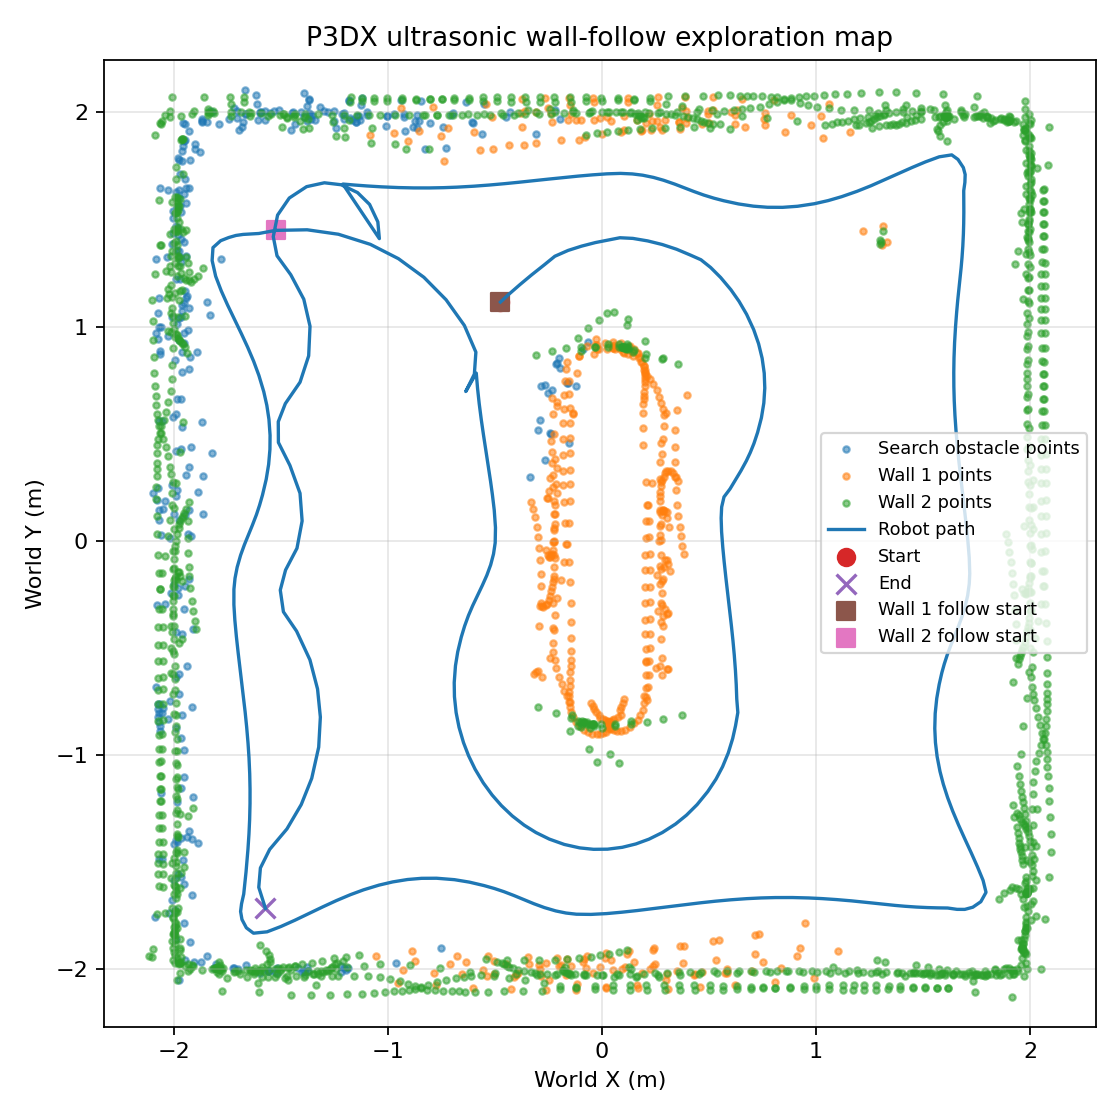
\includegraphics[width=0.78\linewidth]{map_graph.png}}{\fbox{\parbox{0.70\linewidth}{File map\_graph.png belum tersedia.}}}
    \caption{Hasil pemetaan area menggunakan sensor ultrasonik.}
    \label{fig:mapping-result}
\end{figure}

Pada hasil pemetaan terlihat bahwa dinding luar dapat terdeteksi dengan cukup jelas oleh sensor ultrasonik. Selain itu, terdapat obstacle atau dinding di bagian tengah arena yang juga terdeteksi, walaupun jumlah titiknya lebih sedikit dibanding dinding luar. Hal ini menunjukkan bahwa robot lebih banyak menghabiskan waktu mengikuti dinding luar dibanding mengeksplorasi obstacle tengah.

Jika tersedia hasil pemetaan terbaru, gambar berikut dapat digunakan sebagai perbandingan:

\begin{figure}[H]
    \centering
    \IfFileExists{map_graph_final.png}{\includegraphics[width=0.78\linewidth]{map_graph_final.png}}{\IfFileExists{map_graph(1).png}{\includegraphics[width=0.78\linewidth]{map_graph(1).png}}{\fbox{\parbox{0.70\linewidth}{File map\_graph\_final.png belum tersedia.}}}}
    \caption{Hasil pemetaan setelah proses penalaan algoritma wall following.}
    \label{fig:mapping-final}
\end{figure}

\section{Analisis Hasil}

Berdasarkan hasil pemetaan, sistem sudah mampu membaca data ultrasonik, menyimpan titik obstacle, dan menggambarkan peta area dalam bentuk grafik. Dinding luar arena dapat terbentuk dengan cukup baik pada grafik. Namun, lintasan robot masih belum selalu sejajar dengan bentuk dinding. Jalur robot pada beberapa bagian masih membentuk gelombang besar, sehingga dapat disimpulkan bahwa algoritma wall following masih membutuhkan penalaan lebih lanjut.

Beberapa penyebab utama dari masalah tersebut adalah:

\begin{enumerate}[itemsep=0.2em]
    \item Kontrol wall following masih menggunakan aturan sederhana sehingga robot mudah berosilasi.
    \item Sensor ultrasonik memiliki area deteksi yang lebar, sehingga titik obstacle memiliki sebaran yang cukup besar.
    \item Robot belum menggunakan metode SLAM penuh, sehingga belum ada koreksi peta berdasarkan posisi yang lebih akurat.
    \item Dinding luar yang besar dapat membuat robot terlalu lama mengikuti dinding yang sama, sehingga obstacle tengah kurang dieksplorasi.
\end{enumerate}

Untuk meningkatkan performa, beberapa perbaikan yang dapat dilakukan adalah:

\begin{enumerate}[itemsep=0.2em]
    \item Menggunakan kontrol proporsional-derivatif agar robot lebih stabil saat mengikuti dinding.
    \item Menggunakan sensor samping murni untuk menjaga jarak dinding dan sensor diagonal depan untuk mendeteksi sudut.
    \item Membuat logika pencarian obstacle tengah setelah loop dinding luar selesai.
    \item Menggunakan grid occupancy map agar peta lebih mudah dianalisis.
    \item Menambahkan LiDAR virtual jika diizinkan, atau menambahkan sensor proximity tambahan untuk meningkatkan resolusi pemetaan.
\end{enumerate}

\section{Pengujian Sistem dengan Kilo Code}

Pengujian dilakukan dengan menuliskan perintah melalui Kilo Code pada VS Code. Contoh perintah yang digunakan adalah:

\begin{lstlisting}[style=bashstyle]
coppeliasim: go to the target
coppeliasim: mapping the area
coppeliasim: make a counter clockwise circle with 0.5 meter diameter
\end{lstlisting}

Ketika perintah diawali dengan \texttt{coppeliasim:}, Kilo menjalankan \texttt{kilo\_robot\_runner.py}. Program tersebut kemudian menjalankan \texttt{agent\_manager.py} untuk memilih misi yang sesuai. Setelah misi selesai, khusus untuk misi mapping, program membuka file \texttt{map\_graph.png} sebagai hasil pemetaan.

\section{Kesimpulan}

Proyek ini berhasil membuat sistem kontrol robot P3DX berbasis CoppeliaSim yang dapat menerima perintah bahasa natural melalui Kilo Code dan menerjemahkannya menjadi misi robot. Sistem telah mendukung navigasi ke target, obstacle avoidance, pemetaan area menggunakan ultrasonik, dan visualisasi hasil mapping dalam bentuk grafik.

Pendekatan LLM sebagai penerjemah misi terbukti lebih aman dibanding memberikan kendali motor langsung kepada LLM. Dengan arsitektur ini, LLM hanya memilih misi yang tersedia, sedangkan eksekusi gerak tetap dikendalikan oleh algoritma Python yang deterministik. Hasil pemetaan menunjukkan bahwa robot sudah mampu mendeteksi dinding luar dan sebagian obstacle tengah, tetapi algoritma wall following masih perlu ditingkatkan agar lintasan robot lebih mengikuti bentuk dinding secara konsisten.

\section{Lampiran: Contoh Perintah}

\begin{lstlisting}[style=bashstyle]
python agent_manager.py "go to the target"
python agent_manager.py "mapping the area"
python kilo_robot_runner.py "coppeliasim: mapping the area"
python p3dx_interface.py get-state
python p3dx_interface.py apply-action '{"type":"stop"}'
\end{lstlisting}

\end{document}
